\documentclass[resume]{subfiles}


\begin{document}
\begin{multicols}{3}
\section{Circuits}
\subsection{single-supply, inverting, avec référence}
\begin{center}
\includegraphics[scale=1,page=15]{../KiCad/resume-crop.pdf}
\end{center}
$$\boxed{U_{out}=-\frac{R_2}{R_1}\left(U_{in}-U_{ref}\right)+U_{ref}}$$
\subsection{single-supply, non-inverting, sans référence}
\begin{center}
\includegraphics[scale=1,page=16]{../KiCad/resume-crop.pdf}
\end{center}
$$\boxed{U_{out}=\left(1+\frac{R_2}{R_1}\right)\left(U_{in}+U_{ref}\right)+U_{ref}}$$
\subsection{Single supply, differential, avec référence}
\begin{center}
\includegraphics[scale=1,page=5]{../KiCad/resume-crop.pdf}
\end{center}
$$\boxed{U_{out}=\frac{R_2}{R_1}\left(U_{in}-U_{in_{inv}}\right)+U_{ref}}$$
\subsection{Single supply, non inverting, unity gain, avec référence}
\begin{center}
\includegraphics[scale=1,page=3]{../KiCad/resume-crop.pdf}
\end{center}
$$\boxed{U_{out}=\left(U_{in}-U_{ref}\right)+\frac{R_1+R_2}{R_2}U_{ref}}$$
Ou, équivalent :
$$\boxed{U_{out}=\frac{U_{in}R_2+U_{ref}R_1}{R_2}}$$
\subsection{Single supply, inverseur, avec référence}
\begin{center}
\includegraphics[scale=1,page=4]{../KiCad/resume-crop.pdf}
\end{center}
$$\boxed{U_{out}=\frac{U_{ref}R_1-U_{in}R_2}{R_1}}$$
\section{Autres}
\subsection{Statistiques}
\begin{figure}[H]
\centering
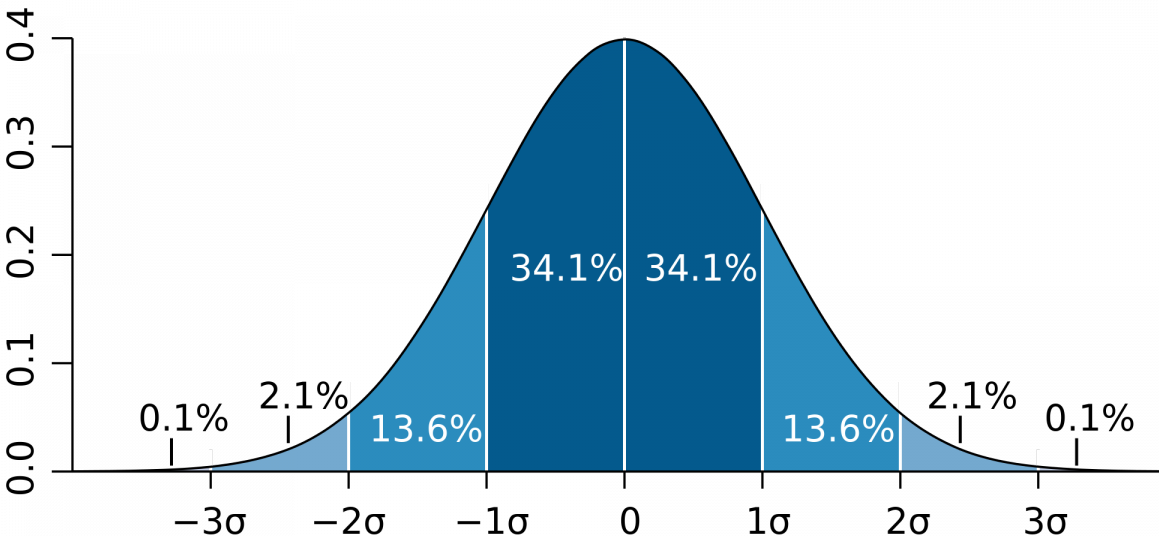
\includegraphics[width=0.6\columnwidth]{gauss.png}
\end{figure}
\subsubsection{Bruit}
Si un bruit est \textbf{aléatoire} (gaussienne), on peut estimer que le \SI{99.9}{\percent} est compris entre $\pm 3.3\sigma$, il est donc possible de passer de pic-pic à rms en multipliant par $2\cdot 3.3$. La valeur rms est $1\sigma$
$$U_{\text{noise}_{pk-pk}}=6.6 U_{\text{noise}_{rms}}$$
\end{multicols}

\end{document}